%\newpage
\section{Notations}
\label{sec:not}
% \subsection{}
In this paper, a graph with node features is denoted as $\mathcal{G}=(\mathbf{X}, \mathbf{A})$, where $\mathcal{V}$ is the vertex set, $\mathcal{E}$ is the edge set, and $\mathbf{X} \in \mathbb{R}^{n \times d_{x}}$ is the feature matrix (\ie, the $i$-th row of $\mathbf{X}$ is the feature vector $\mathbf{x}_i$ of node $v_{i}$) and $\mathbf{A} \in\{0,1\}^{n \times n}$ denotes the adjacency matrix of $G$, \ie, the $(i, j)$-th entry in $\mathbf{A}$ is 1 if there is an edge between $v_{i}$ and $v_{j}$.
%
The degree of node $v_{i}$, denoted as $d_{i}$, is the number of edges incident with $v_{i}$.
%
The degree matrix $\mathbf{D}$ is a diagonal matrix and its $i$-th diagonal entry is $d_{i}$. 
%
For a $d$-dimensional vector $\mathbf{x} \in \mathbb{R}^{d}, \|\mathbf{x}\|_{2}$ is the Euclidean norm of $\mathbf{x}$.
%
We use ${x}_{i}$ to denote the $i$ th entry of $\mathbf{x}$, and $\operatorname{diag}(\mathbf{x}) \in \mathbb{R}^{d \times d}$ is a diagonal matrix such that the $i$-th diagonal entry is $x_{i}$. 
%
We use $\mathbf{a}_{i}$ denote the row vector of $\mathbf{A}$ and ${a}_{ij}$ for the $(i, j)$-th entry of $\mathbf{A}$. 
%
The trace of a square matrix $\mathbf{A}$ is denoted by $\operatorname{Tr}(\mathbf{A})$, which is the sum along the diagonal of $\mathbf{A}$. 
%
% The singular value decomposition of $\mathbf{A}$ is denoted as $\mathbf{A} = \mathbf{U}\mathbf{\Sigma}\mathbf{V}^\top$ where $\mathbf{U}=\left[\mathbf{u}_{1}, \ldots, \mathbf{u}_{n}\right], \mathbf{\Sigma}=\operatorname{diag}\left (\sigma_{1}, \ldots, \sigma_{d}\right)$, and $\mathbf{V}=\left[\mathbf{v}_{1}, \ldots, \mathbf{v}_{d}\right]$. 
%
We use $\| \mathbf{A} \|_2$ to denote the spectral norm of $\mathbf{A}$, which is its largest singular value $\sigma_{\max}$. 
%
We use $\|\mathbf{A}\|_F$ for the Frobenius Norm, which is $\|\mathbf{A}\|_{\mathrm{F}}=\sqrt{\sum_{i,j}\left|a_{i j}\right|^{2}}=\sqrt{\operatorname{
Tr}\left(\mathbf{A^\top A}\right)}$.
% =\sqrt{\sum_{i=1}^{d} \sigma_{i}^{2}(\mathbf{A})}$.

% \subsection{Proofs of Theorem~\ref{theorem:gb}}
% \begin{definition}~\citelatex{DBLP:journals/corr/abs-2111-00743}
%  $((\sigma, \delta)$-Augmentation). The data augmentation set $A$ is called a $(\sigma, \delta)$-augmentation, if for each class $C_{k}$, there exists a subset $C_{k}^{0} \subseteq C_{k}$ (called the main part of $C_{k}$ ) such that the following two conditions hold: 1) $\mathbb{P}\left[\mathbf{x} \in C_{k}^{0}\right] \geq \sigma \mathbb{P}\left[\mathbf{x} \in C_{k}\right]$ where $\sigma \in(0,1]$, 2) $\sup _{\mathbf{x}_{1}, \mathbf{x}_{2} \in C_{k}^{0}} d_{A}\left(\mathbf{x}_{1}, \mathbf{x}_{2}\right) \leq \delta$.
% \end{definition}


% \begin{lemma}~\citelatex{DBLP:journals/corr/abs-2111-00743}
% For a $(\sigma, \delta)$-augmentation with main part $C_{k}^{0}$ of each class $C_{k}$, if all samples belonging to $\left(C_{1}^{0} \cup \cdots \cup C_{K}^{0}\right) \cap S_{\varepsilon}$ can be correctly classified by a classifier $G$, then its downstream error rate $\operatorname{Err}(G) \leq$ $(1-\sigma)+R_{\varepsilon}$. $R_{\varepsilon}:=\mathbb{P}\left[{S_{\varepsilon}}\right]$ and $S_{\varepsilon}:=\{\mathbf{x} \in \cup_{k=1}^{K} C_{k}: \forall \mathbf{x}_{1}, \mathbf{x}_{2} \in A(\mathbf{x}),\left\|f\left(\mathbf{x}_{1}\right)-f\left(\mathbf{x}_{2}\right)\right\| \geq \varepsilon\}$.
% \end{lemma}
% Because $\left\|f\left(\mathbf{x}_{1}\right)-f\left(\mathbf{x}_{2}\right)\right\|$ is a non-negative random variable. Then, for any $\epsilon>0$, according to markov inequality we have:
% \begin{equation}
% \mathbb{P}[\left\|f\left(\mathbf{x}_{1}\right)-f\left(\mathbf{x}_{2}\right)\right\|_2^2 \geq \epsilon^2 ] \leq \frac{\mathbb{E}_{\mathbf{x}_{1}, \mathbf{x}_{2} \in A(\mathbf{x})}[\left\|f\left(\mathbf{x}_{1}\right)-f\left(\mathbf{x}_{2}\right)\right\|_2^2]}{\epsilon^2}.
% \end{equation}
% Here we let $f(\mathbf{x})=1$ and $\mathbb{E}_{\mathbf{x}_{1}, \mathbf{x}_{2} \in A(\mathbf{x})}[\left\|f\left(\mathbf{x}_{1}\right)-f\left(\mathbf{x}_{2}\right)\right\|_2^2] = 2 - 2\mathbb{E}_{\mathbf{x}_{1}, \mathbf{x}_{2} \in A(\mathbf{x})}[f\left(\mathbf{x}_{1}\right)^\top f\left(\mathbf{x}_{2}\right)]=2-2\mathcal{L}_{a}$.

\section{Bounded Noise Matrix.}
% \label{sec:improveAligment}
For completeness, we  analyze the relation between the orthonormal bases $\  {\mathbf{V}}$ and $\mathbf{V}$ of   $\widetilde{\mathbf{H}}$ and $\mathbf{H}$, the augmentation error bounded by $\eta$, and the distribution of the spectrum. Let $\mathbf{E} = |\widetilde{\mathbf{H}} - \mathbf{H}|$ be  the absolute error matrix where $\mathbf{E}_{ij} = |\widetilde{\mathbf{H}}_{ij} - \mathbf{H}_{ij}| \leq \eta$. Let $\{\widetilde{\sigma}_i\}$ and $\{\sigma_i\}$ be sets of singular values of $\widetilde{\mathbf{H}}$ and $\mathbf{H}$. We derive the following bound.
\begin{proposition}
\label{prop:ebound}
If %the difference of 
$\|\mathbf{V}\!-\!\widetilde{\mathbf{V}}\|_2\!\leq\!\epsilon$,  each element in $\mathbf{E}_{ij}$ (the absolute error) is bounded by %$\eta$ and 
%$\tau \leq 2 \varepsilon d_{1} /(N(\pi+2 \varepsilon))$. 
$\eta = 2 \varepsilon\Delta\tilde{\sigma}_{12} /(n\pi+2\varepsilon)$, where $n$ is the number of nodes and $\Delta\tilde{\sigma}_{12}=\widetilde{\sigma}_1-\widetilde{\sigma}_2$ is the singular value gap  of $\widetilde{\mathbf{H}}$.
\end{proposition}
\vspace{-1cm}
\begin{proof}
See \nameref{proof:ebound} (suppl. material).
\end{proof}

%\begin{remark}
%We observe from the feature space that our method adds an adaptive noise to the original features. In the above theorem, we show that the absolute error of each element in the noise matrix is bounded and is highly related to the singular value gap, which controls the intensity of augmentation.
%\end{remark}


%\definecolor{LightCyan}{rgb}{0.88,1,1}
\definecolor{beaublue}{rgb}{0.88,1,1}
\definecolor{blackish}{rgb}{0.2, 0.2, 0.2}
\begin{tcolorbox}[width=1.0\linewidth, colframe=blackish, colback=beaublue, boxsep=0mm, arc=2mm, left=2mm, right=2mm, top=2mm, bottom=2mm]
%\begin{tcolorbox}[colframe=black]
 Prop. \ref{prop:ebound} shows that the absolute difference between the augmented and  original feature matrices is bounded (variance in Prop. \ref{prop:PowerIterVar} does not guarantee that). Moreover, as Prop. \ref{prop:PowerIter1} shows the flattening of spectrum indeed takes place, this means that the spectral gaps $\Delta\tilde{\sigma}^\alpha_{12}$ and $\Delta\tilde{\sigma}^\beta_{12}$ of both augmented feature matrices   $\widetilde{\mathbf{H}}^\alpha$ and $\widetilde{\mathbf{H}}^\beta$ from both views are bounded and limited compared to the spectral gaps of original matrices ${\mathbf{H}}^\alpha$ and ${\mathbf{H}}^\beta$. The profound consequence of this observation is that $\widetilde{\mathbf{V}}^\alpha$ and $\widetilde{\mathbf{V}}^\beta$ are then closer to original ${\mathbf{V}}^\alpha$ and ${\mathbf{V}}^\beta$, and so the angle alignment between of two views enjoys an improved quality.  
%
%we conclude that by injecting the noise into the spectrum, we obtain the augmented features $\widetilde{\mathbf{H}}$ whose orthonormal basis remains unchanged with the original orthonormal basis of  ${\mathbf{H}}$, \ie, the directions of singular vectors of $\widetilde{\mathbf{H}}$ and ${\mathbf{H}}$ are aligned but the spectra of $\widetilde{\mathbf{H}}$ and ${\mathbf{H}}$ differ. In contrast, injecting the random noise  or applying dropout on ${\mathbf{H}}$ would perturb its orthonormal basis.
\end{tcolorbox}

\section{Proofs of Propositions}

Below we present proofs for several propositions that were not included in the main draft. % for brevity.

\setcounter{subsection}{1}
\subsection{Proof of Proposition \ref{prop:FeatureAug}}

\begin{proof}
Let $\mathbf{H} = \mathbf{U} \boldsymbol{\Sigma} \mathbf{V}^{\top}$ be the SVD of an input feature map, where $\mathbf{U}$ and $\mathbf{V}$ are the right and left orthonormal matrices that contain the singular vectors. As $\mathbf{r}^{(k)} = (\mathbf{H}^\top\mathbf{H})^k\mathbf{r}^{(0)}$, we have: % the following:
\begin{equation}
    \mathbf{r}^{(k)} = (\mathbf{H}^\top\mathbf{H})^{k}\mathbf{r}^{(0)} = (\mathbf{V}\boldsymbol{\Sigma}^{2k} \mathbf{V}^{\top})\mathbf{r}^{(0)}.
    \label{equ:Iter}
\end{equation}
Plugging Equation~(\ref{equ:Iter}) into Equation~(\ref{equ:FeatureAug}), we obtain:
\begin{equation}
\begin{aligned}
        \!\!\!\!\frac{\mathbf{H} \mathbf{r}^{(k)} \mathbf{r}^{(k)\top}}{\|\mathbf{r}^{(k)}\|_2^2} &\!=\! \frac{\mathbf{U}\Sigma\mathbf{V}^\top (\mathbf{V}\boldsymbol{\Sigma}^{2k} \mathbf{V}^{\top})\mathbf{r}^{(0)} \mathbf{r}^{(0)\top}(\mathbf{V}\boldsymbol{\Sigma}^{2k} \mathbf{V}^{\top})}{\mathbf{r}^{0}(\mathbf{V}\boldsymbol{\Sigma}^{2k} \mathbf{V}^{\top})(\mathbf{V}\boldsymbol{\Sigma}^{2k} \mathbf{V}^{\top})\mathbf{r}^{0}}\\
        &\!=\! \frac{\mathbf{U}\boldsymbol{\Sigma}^{2k+1} \mathbf{V}^{\top}\mathbf{r}^{(0)} \mathbf{r}^{(0)\top}\mathbf{V}\boldsymbol{\Sigma}^{2k} \mathbf{V}^{\top}}{\mathbf{r}^{(0)\top}\mathbf{V} \Sigma^{4k} \mathbf{V}^{\top}\mathbf{r}^{(0)}}.\!\!
        \label{eq:com}
\end{aligned}
\end{equation}
Let $\mathbf{y} = \mathbf{V}^{\top}\mathbf{r}^{(0)}$ and $k\geq1$ be the number of iterations, then we simplify Eq.~\eqref{eq:com} as:
%\begin{equation}
%\!\!\!\!\!\!\!\!
\begin{align}
        &\frac{\mathbf{H} \mathbf{r}^{(k)} \mathbf{r}^{(k)\top}}{\|\mathbf{r}^{(k)}\|_2^2} \!=\!\mathbf{U}\mathbf{Q}(\mathbf{y},k)\mathbf{V}^\top\\
        \text{ where }\;& \mathbf{Q}(\mathbf{y},k)\!=\!\frac{\boldsymbol{\Sigma}^{2k+1}\mathbf{y}\mathbf{y}^\top\boldsymbol{\Sigma}^{2k}}{\mathbf{y}^\top\boldsymbol{\Sigma}^{4k}\mathbf{y}}.
        \label{eq:sim}
\end{align}
%\end{equation}
As $\mathbf{r}^{(0)} \sim \mathcal{N}(0,\mathbf{I})$ and $\mathbf{V}$ is a unitary matrix, we have $\mathbf{y}=[y_1,\cdots,y_{d_h}]\sim\mathcal{N}(0, \mathbf{I})$. The expectation of $\mathbf{Q}$ % = \frac{\Sigma^{2k+1}\mathbf{y}\mathbf{y}^\top\Sigma^{2k}}{\mathbf{y}^\top\Sigma^{4k}\mathbf{y}}$ %
is a diagonal matrix, \ie, we have $\mathbb{E}_{\mathbf{y}\sim\mathcal{N}(0, \mathbf{I})}(\mathbf{Q}(\mathbf{y},k)) = \text{diag}\big(q_1(k), q_2(k), \cdots, q(k)_{d_h}\big)$ with:

\vspace{-0.3cm}
\begin{equation}
\begin{aligned}
\label{eq:balanceq}
    q_{i}(k)=\sigma_{i} \lambda_{i}(k)  &\text{ where }  \lambda_{i}(k)=\mathbb{E}_{\mathbf{y}\sim\mathcal{N}(0;\mathbf{I})}\big(\lambda'_i(\mathbf{y},k)\big), \; \\
    &{\text{ and }} \lambda'_i(\mathbf{y},k)=
    \text{\fontsize{8}{8}\selectfont$\frac{\left(y_{i} \sigma_{i}^{2k}\right)^{2}}{ \sum_{l=1}^{d_h}\left(y_{l} \sigma_{l}^{2k}\right)^{2}}$}.
    %  \text{ and } \mathbf{y}=[y_1,\cdots,y_{d_h}].
    %=\sigma_{i} \lambda_{i}.
    \end{aligned}
\end{equation}
For brevity, let us drop parameter $k$ where possible. We need to show that $1 \geq \lambda_i \geq \lambda_j\geq 0$ when $\sigma_i \geq \sigma_j$. Obviously, $1 \geq\lambda_i\geq0$, thus we need to show that $\lambda_i-\lambda_j\geq 0$ (note\footnote{Each expectation in Equation \eqref{eq:balance} runs over ${\mathbf{y}\sim\mathcal{N}(0;\mathbf{I})}$, that is, $\mathbb{E}_{\mathbf{y}\sim\mathcal{N}(0;\mathbf{I})}(\cdot)$.}):
\begin{equation}
% %\begin{aligned}
% \label{eq:balance}
%           \lambda_i - \lambda_j = \text{\fontsize{8}{8}\selectfont$\mathbb{E}\left(\frac{\left(y_{i} \sigma_{i}^{2k}\right)^{2}}{ \sum_{l=1}^{d_h}\left(y_{l} \sigma_{l}^{2k}\right)^{2}}\right)-\mathbb{E}
%           \Bigg(\frac{\big(y_{j} \sigma_{j}^{2k}\big)^{2}}{ \sum_{l=1}^{d_h}\left(y_{l}\sigma_{l}^{2k}\right)^{2}}\Bigg)
%           \geq \sigma_{j}^{4k} \mathbb{E}\left(\frac{y^{2}_i - y^{2}_j}{ \sum_{l=1}^{d_h}\left(y_{l} \sigma_{l}^{2k}\right)^{2}}\right) = 0.$}
% %\end{aligned}
\label{eq:balance}
\begin{aligned}
          \lambda_i - \lambda_j =& \mathbb{E}\left(\frac{\left(y_{i} \sigma_{i}^{2k}\right)^{2}}{ \sum_{l=1}^{d_h}\left(y_{l} \sigma_{l}^{2k}\right)^{2}}\right)-\mathbb{E}
          \Bigg(\frac{\big(y_{j} \sigma_{j}^{2k}\big)^{2}}{ \sum_{l=1}^{d_h}\left(y_{l}\sigma_{l}^{2k}\right)^{2}}\Bigg)\\
          &\geq \sigma_{j}^{4k} \mathbb{E}\left(\frac{y^{2}_i - y^{2}_j}{ \sum_{l=1}^{d_h}\left(y_{l} \sigma_{l}^{2k}\right)^{2}}\right) = 0.
\end{aligned}
\end{equation}


As $$\mathbb{E}_{\mathbf{y}\sim\mathcal{N}(0;\mathbf{I})}\!\left(\frac{y^{2}_i - y^{2}_j}{ \sum_{l=1}^{d_h}\left(y_{l} \sigma_{l}^{2k}\right)^{2}}\right)=$$ 
%
 $$\mathbb{E}_{\mathbf{y}\sim\mathcal{N}(0;\mathbf{I})}\!\left(\frac{y^{2}_i}{ \sum_{l=1}^{d_h}\left(y_{l} \sigma_{l}^{2k}\right)^{2}}\right)\!-\!
  \mathbb{E}_{\mathbf{y}\sim\mathcal{N}(0;\mathbf{I})}\!\left(\frac{y^{2}_j}{ \sum_{l=1}^{d_h}\left(y_{l} \sigma_{l}^{2k}\right)^{2}}\right)
 %
 %
\!=\!0$$ 

\noindent
due to
  $y_i$, $y_j$ being i.i.d. random variables sampled from the normal distribution,  inequality \eqref{eq:balance} holds. % a Above derivations complete the proof.
\end{proof}




\subsection{Proof of Proposition \ref{prop:PowerIter1}}
\label{exp_val}
\begin{proof}[Proof]
We split the proof into four steps as follows.


\vspace{0.1cm}\noindent
\textbf{Step 1.} 
Let $\beta_i=(\sigma_i^{2k})^2$.  Define random variable $x_i(\mathbf{y})=\frac{\beta_i y_{i}^2}{\beta_i y_{i}^2 +\sum_{l\neq i}\beta_l y^2_{l} }=\frac{y_{i}^2}{y_{i}^2 +\sum_{l\neq i}\frac{\beta_l}{\beta_i}y^2_{l} }=\frac{u}{u+v_i}$ where ${\mathbf{y}\sim\mathcal{N}(0;\mathbf{I})}$, $u=y_i^2$ and $v_i=\sum_{l\neq i}\frac{\beta_l}{\beta_i}y^2_{l}$. Notice that transformation $y_i^2$ of the random variable ${{y_i}\sim\mathcal{N}(0;1)}$ in fact $\chi^2(1)$ distributed, \ie, $y_i^2\sim\chi^2(1)=\mathcal{G}(\frac{1}{2},2)$ because $\chi^2(t)\equiv\mathcal{G}(\frac{t}{2},2)$ (it is a well-known fact that the $\chi^2(t)$ is a special case of the Gamma distribution defined with the scale parameter).

\vspace{0.1cm}\noindent
\textbf{Step 2.} 
Next, finding the exact distribution of $v_i$ (a weighted sum of chi squares) is a topic of ongoing studies but highly accurate surrogates exist, \ie, authors of \citelatex{weighted_chi_squares_sup} show that   $\sum_l\zeta_l y_l^2\sim\mathcal{G}\Big(\frac{1}{2}\frac{(\sum_l\zeta_l)^2}{\sum_l\zeta_l^2}, 2\frac{\sum_l\zeta_l^2}{\sum_l \zeta_l} \Big)$ for weights $\zeta_l\geq 0$ and $\sum_l \zeta_l>0$, and so we have 
$v_i\sim\mathcal{G}\Big(\frac{1}{2}\frac{(\sum_{l\neq i}\beta_l)^2}{\sum_{l\neq i}\beta_l^2}, \frac{2}{\beta_i}\frac{\sum_{l\neq i}\beta_l^2}{\sum_{l\neq i} \zeta_l} \Big)$.

\vspace{0.1cm}\noindent
\textbf{Step 3.} 
Now, our proof requires determining the distribution of $x_i=\frac{u}{u+v_i}$ where $u\sim\mathcal{G}(\alpha_0,\theta_0)=\mathcal{G}(\frac{1}{2},2)$ and $v_i\sim\mathcal{G}(\alpha_i,\theta_i)=\mathcal{G}\Big(\frac{1}{2}\frac{(\sum_{l\neq i}\beta_l)^2}{\sum_{l\neq i}\beta_l^2}, \frac{2}{\beta_i}\frac{\sum_{l\neq i}\beta_l^2}{\sum_{l\neq i} \zeta_l} \Big)$. Let $x=\frac{u}{u+v}=\frac{1}{1+b}$ for $u\sim\mathcal{G}(\alpha_0,\theta)$ and $v\sim\mathcal{G}(\alpha_i,\theta)$, then  the following are well-known results that  $x\sim\mathcal{B}(\alpha_0,\alpha_i)$  and $b=u/v\sim\mathcal{B}'(\alpha_i,\alpha_0)$ where $\mathcal{B}$ and $\mathcal{B}'$ stand for the Beta distribution and the Standard Beta Prime distribution, respectively. Let $x_i=\frac{u}{u+v_i}=\frac{1}{1+\gamma_i b_i},\;0\leq\gamma_i\leq\infty$ where $\gamma_i=\frac{\theta_i}{\theta_0}$ (ratio of scalars in Gamma distributions, \ie, $v_i\sim\mathcal{G}(\alpha_i,\theta_i)$)  and $b_i=\frac{1-x_i}{x_i}$ (solving $x_i=\frac{1}{1+b_i}$ for $b_i$). Substituting $b_i=\frac{1-x_i}{x_i}$ into $\frac{1}{1+\gamma_i b_i}$ yields $z=\frac{x_i}{\gamma_i+(1-\gamma_i)x_i}$ and since we have to perform the change of variable, we compute (i) $x_i=\frac{\gamma_i z}{1-(1-\gamma_i)z}$ and (ii) the Jacobian which takes a simple form $\frac{\partial x_i}{\partial z}=\frac{\gamma_i}{(\gamma_i+(1-\gamma_i)z)^2}$. Finally, we have $x^\bullet_i(z)= \mathcal{B}(x_i; \alpha_0,\alpha_i)\cdot\lvert\frac{\partial x_i}{\partial z}\rvert=\frac{\gamma_i}{(\gamma_i+(1-\gamma_i)z)^2}\cdot\mathcal{B}\left(\frac{\gamma_i z}{1-(1-\gamma_i)z}; \alpha_0,\alpha_i\right)$. As $\alpha_0=\frac{1}{2}$ and $\theta_0=2$, we have $\gamma_i=\frac{1}{\beta_i}\frac{\sum_{l\neq i}\beta_l^2}{\sum_{l\neq i} \zeta_l} $, $\theta_i=2\gamma_i$ (following our earlier assumptions on modeling $v_i$), and the PDF underlying our spectrum-balancing algorithm is $x^\bullet_i(z)=\frac{\gamma_i}{(\gamma_i+(1-\gamma_i)z)^2}\cdot\mathcal{B}\Big(\frac{\gamma_i z}{1-(1-\gamma_i)z}; \frac{1}{2},\alpha_i\Big)$. Moreover, the above PDF enjoys the support $z\in[0 ;1]$ because $\mathcal{B}(x_i)$ enjoys the support $x_i\in[0 ;1]$ and function $x_i: [0 ;1]\longmapsto[0 ;1]$.

\vspace{0.1cm}\noindent
\textbf{Step 4.} 
Finally, $\lambda_i=\mathbb{E}(z)=\int_0^1 z\cdot x^\bullet_i(z) \, \mathrm{d}z$ is simply obtained by the integration using the Mathematica software followed by a few of algebraic simplifications regarding switching the so-called regularized Hypergeometric function with the so-called Hypergeometric function.
\end{proof}

\subsection{Proof of Proposition \ref{prop:PowerIterVar}}
\label{exp_var}
\begin{proof}[Proof]
Variance $\omega^2_i=\mathbb{E}(z^2)-(\mathbb{E}(z))^2=\int_0^1 z^2\cdot x^\bullet_i(z) \, \mathrm{d}z - \lambda^2_i$ relies on the PDF expression $x^\bullet_i(z)$ derived in the Proof \ref{exp_val}. Expression $\int_0^1 z^2\cdot x^\bullet_i(z) \, \mathrm{d}z$ is simply obtained by the integration using the Mathematica software  followed by a few of algebraic simplifications regarding switching the so-called regularized Hypergeometric function with the so-called Hypergeometric function.
\end{proof}

\subsection{Proof of Proposition~\ref{prop:ebound}}
\label{proof:ebound}
\begin{proof}[Proof]
Since $\|\mathbf{E}\|_2^2 \leq \|\mathbf{E}\|^2_F \leq n^2 \tau^2$, we have:
\begin{equation}
\label{equ:nbequ0}
    \|\mathbf{E}\|_2 \leq n\tau.
\end{equation}
From works~\citelatex{kostrykin2003subspace_sup,wang2008manifold_sup}, we know that if $\widetilde{\mathbf{H}}$ and $\mathbf{E}$ are self-adjoint operators on a separable Hilbert space, then the spectrum of $\mathbf{H}$ is in the closed $\|\mathbf{E}\|-$neighborhood of the spectrum of $\widetilde{\mathbf{H}}$. Thus, we have the following inequality:
\begin{equation}
\label{equ:nbequ}
    \|\mathbf{V}^{\perp} \mathbf{V}'\|_2 \leq \pi\|\mathbf{E}\|_2/2\Delta\tilde{\sigma},
\end{equation}
% where $d = |\widetilde{\sigma}_1 - \sigma_2|$. 
As we know $\widetilde{\mathbf{H}}$ has the singular value gap $\Delta\tilde{\sigma}_{12}$
% =|\widetilde{\sigma}_1 - \widetilde{\sigma}_2|$. 
We need to assume $\|\mathbf{E}\|_2<\Delta\tilde{\sigma} / 2$ to guarantee $\mathbf{H}$ also has the singular value gap. Thus, Equation~(\ref{equ:nbequ}) becomes:
\begin{equation}
\label{equ:nbequ2}
    \|\mathbf{V}^{\perp} \widetilde{\mathbf{V}}\|_2 \leq \pi\|\mathbf{E}\|_2/2(\Delta\tilde{\sigma}_{12}-\|\mathbf{E}\|_2).
\end{equation}
Similarly, we also have:
\begin{equation}
\label{equ:nbequ3}
    \|\mathbf{V}\widetilde{\mathbf{V}}^{\perp}\|_2 \leq \pi\|\mathbf{E}\|_2/2(\Delta\tilde{\sigma}_{12}-\|\mathbf{E}\|_2).
\end{equation}
Since $\|\mathbf{V}-\widetilde{\mathbf{V}}\|_2 = \max(\|\mathbf{V}\widetilde{\mathbf{V}}^{\perp}\|_2,\|\mathbf{V}^{\perp}\widetilde{\mathbf{V}}\|_2)$, we have the following bound:
\begin{equation}
\label{equ:bound}
    \|\mathbf{V}-\widetilde{\mathbf{V}}\|_2  \leq \pi\|\mathbf{E}\|_2/2(\Delta\tilde{\sigma}_{12}-\|\mathbf{E}\|_2).
\end{equation}
Equation~(\ref{equ:bound}) implies if $\|\widetilde{\mathbf{V}} - \mathbf{V}\|_2<\epsilon$, we get $\|\mathbf{E}\|_2 \leq 2 \Delta\tilde{\sigma}_{12} \varepsilon/(2 \varepsilon+\pi)$. Combined with Equation~(\ref{equ:nbequ0}), we arrive at the conclusion that if the difference of $\|\mathbf{V}-\widetilde{\mathbf{V}}\|_2$ is at most $\epsilon$, the absolute error of each element in $\mathbf{E}$ is bounded by $\tau$ and $\tau \leq 2 \varepsilon \Delta\tilde{\sigma}_{12} /(n(\pi+2 \varepsilon))$.
\end{proof}


\subsection{Proof of Theorem~\ref{theorem:gb}}
\label{gen_bound_proof}
\begin{proof}[Proof]
\begin{definition}~\citelatex{DBLP:journals/corr/abs-2111-00743_sup}
 $((\sigma, \delta)$-Augmentation). The data augmentation set $\mathcal{A}$ is called a $(\sigma, \delta)$-augmentation, if for each class $C_{k}$, there exists a subset $C_{k}^{0} \subseteq C_{k}$ (called the main part of $C_{k}$ ) such that the following two conditions hold: (i) $\mathbb{P}\left[\mathbf{x} \in C_{k}^{0}\right] \geq \sigma \mathbb{P}\left[\mathbf{x} \in C_{k}\right]$ where $\sigma \in(0,1]$, (ii) $\sup _{\mathbf{x}_{1}, \mathbf{x}_{2} \in C_{k}^{0}} d_\mathcal{A}\left(\mathbf{x}_{1}, \mathbf{x}_{2}\right) \leq \delta$.
\end{definition}


\begin{lemma}~\citelatex{DBLP:journals/corr/abs-2111-00743_sup}
For a $(\sigma, \delta)$-augmentation with main part $C_{k}^{0}$ of each class $C_{k}$, if all samples belonging to $\left(C_{1}^{0} \cup \cdots \cup C_{K}^{0}\right) \cap S_{\varepsilon}$ can be correctly classified by a classifier $G$, then its downstream error rate $\operatorname{Err}(G) \leq$ $(1-\sigma)+R_{\varepsilon}$. $R_{\varepsilon}:=\mathbb{P}\left[{S_{\varepsilon}}\right]$ and $S_{\varepsilon}:=\{\mathbf{x} \in \cup_{k=1}^{K} C_{k}: \forall \mathbf{x}_{1}, \mathbf{x}_{2} \in \mathcal{A}(\mathbf{x}),\left\|f\left(\mathbf{x}_{1}\right)-f\left(\mathbf{x}_{2}\right)\right\| \geq \varepsilon\}$.
\end{lemma}
Because $\left\|f\left(\mathbf{x}_{1}\right)-f\left(\mathbf{x}_{2}\right)\right\|$ is a non-negative random variable. Then, for any $\epsilon>0$, according to markov inequality we have:
\begin{equation}
\begin{aligned}
          &\mathbb{P}[\left\|f\left(\mathbf{x}_{1}\right)-f\left(\mathbf{x}_{2}\right)\right\|_2^2 \geq \epsilon^2 ]\\
          &\leq {\mathbb{E}_{\mathbf{x}_{1}, \mathbf{x}_{2} \in \mathcal{A}(\mathbf{x})}[\left\|f\left(\mathbf{x}_{1}\right)-f\left(\mathbf{x}_{2}\right)\right\|_2^2]}/{\epsilon^2}.
\end{aligned}
\end{equation}
Let $f(\mathbf{x})=1$ and  $\mathbb{E}_{\mathbf{x}_{1}, \mathbf{x}_{2} \in \mathcal{A}(\mathbf{x})}[\left\|f\left(\mathbf{x}_{1}\right)-f\left(\mathbf{x}_{2}\right)\right\|_2^2] = 2 - 2\mathbb{E}_{\mathbf{x}_{1}, \mathbf{x}_{2} \in \mathcal{A}(\mathbf{x})}[f\left(\mathbf{x}_{1}\right)^\top f\left(\mathbf{x}_{2}\right)]= 2-2\mathcal{L}_{a}$. And thus we have $R_{\varepsilon}\!\!= \!\!P_{\mathbf{x}_{1}, \mathbf{x}_{2} \in \mathcal{A}(\mathbf{x})}\{\|f\left(\mathbf{x}_{1}\right)\!-\!f\left(\mathbf{x}_{2})\| \!\geq\! \varepsilon\right\}\!\leq\!\frac{\sqrt{2-2\mathcal{L}_{a}}}{\varepsilon}$.
\end{proof}

\subsection{Upper bound of $\phi$}
\label{lambda_upper}
%\begin{proof}[Proof]
As SFA seeks to remove the contribution of the largest singular value of $\mathbf{H}$ from the spectrum $\sigma_1\geq\sigma_2\geq\cdots\geq\sigma_{d_h}$ of $\mathbf{H}$, it follows that for $\sigma_i$ we have the upper bound on the push-forward function such that $\phi(\sigma_i;k)\leq \bar{\phi}(\sigma_i)-\mathcal{O}(k)$ where $\bar{\phi}(\sigma_i)=\min(\sigma_i, \max\limits_{j\neq i}(\sigma_j))$ and $\mathcal{O}(k)\geq 0$.

 Figure \ref{fig:bound} illustrates the above bound. As is clear, the lower the value $k$ is, the more ample is the possibility to tighten that bound (the gap to tighten is captured by $\mathcal{O}(k)\geq0$).

Nonetheless, with this simple upper bound, we show that we clip/balance spectrum and so the loss in Eq. \eqref{equ:EignAlignRefine} enjoys lower energy than the loss in Eq. \eqref{equ:EignAlignOri}, on which  Theorem~\ref{theorem:gb} relies.


\begin{figure}[h]
%\vspace{-0.5cm}
\centering
%\begin{subfigure}[b]{0.32\textwidth}

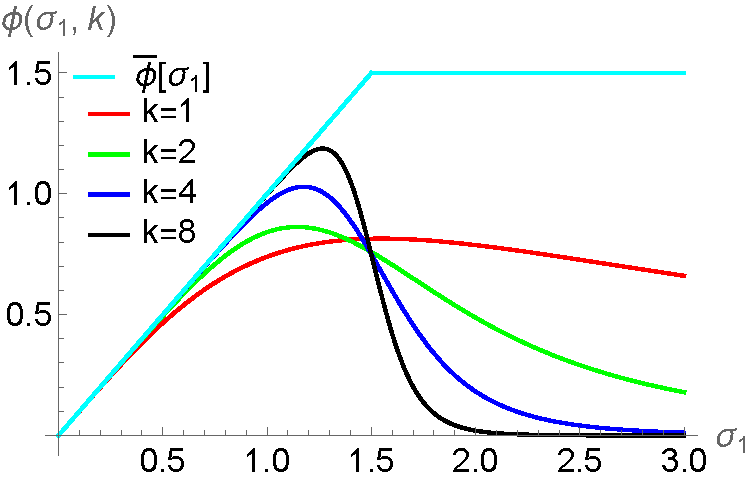
\includegraphics[width=0.3\textwidth]{picture/sim_bound.pdf}
%\caption{\label{fig:bound}  }
%\end{subfigure}
%\begin{subfigure}[b]{0.32\textwidth}
%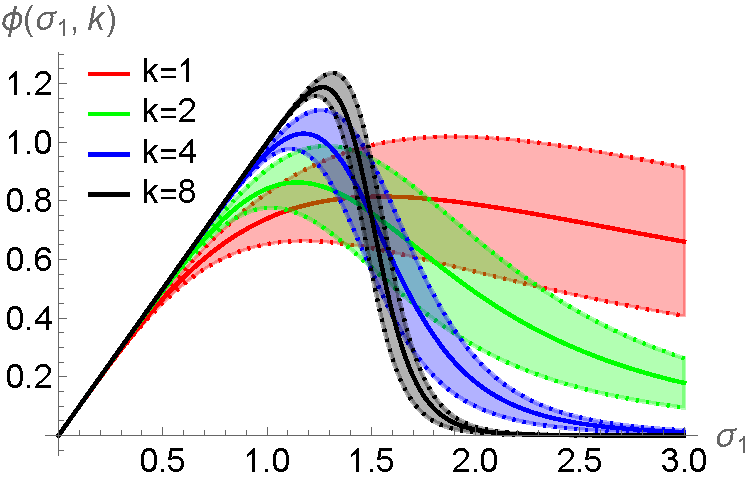
\includegraphics[width=\textwidth]{picture/sim_muvar.pdf}
%\caption{\label{fig:sim2}  }
%\end{subfigure}
%\begin{subfigure}[b]{0.32\textwidth}
%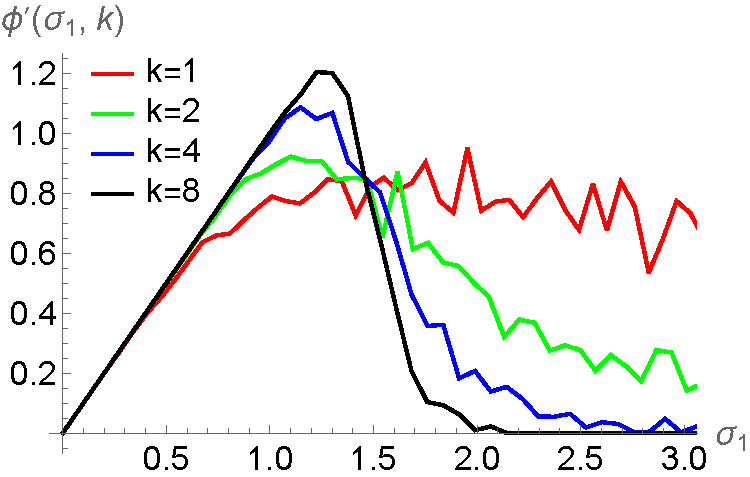
\includegraphics[width=\textwidth]{picture/sim_iter.pdf}
%\caption{\label{fig:sim3}  }
%\end{subfigure}
%\begin{subfigure}[b]{0.24\textwidth}
%\includegraphics[width=\textwidth]{picture/pic4.pdf}
%\caption{\label{fig:sim4} }
%\end{subfigure}
\caption{Illustration of $\phi(\sigma_1;k)$ \vs $\bar{\phi}(\sigma_1)$.}
\label{fig:bound}
\end{figure}

%\end{proof}

Notice that the upper bound in Figure \ref{fig:bound} is also known as the so-called AxMin pooling operator \citelatex{s19_sup}.



\subsection{Derivation of MaxExp(F)}
\label{sec:maxexp}

Derivation of MaxExp(F) in Eq. \eqref{eq:maxexp} is based on the following steps. Based on SVD, we define $\mathbf{H}=\mathbf{U}\mathbf{\Sigma}\mathbf{V}^\top$, where $\mathbf{U}$ and $\mathbf{V}$ are left and right singular vectors of $\mathbf{H}$ and $\mathbf{\Sigma}$ are singular values placed along the diagonal. 

\vspace{0.1cm}
\noindent Let $\mathbf{A}^2\!=\!\mathbf{H}^\top\mathbf{H}\!=\!\mathbf{V}\mathbf{\Sigma}^2\mathbf{V}^\top$ and $\mathbf{A}\!=\!\big(\mathbf{H}^\top\mathbf{H})^{0.5}\!=\!\mathbf{V}\mathbf{\Sigma}\mathbf{V}^\top$. Let  $\mathbf{B}^2\!=\!(\mathbf{H}^\top\mathbf{H})^{-1}\!=\!\mathbf{V}\mathbf{\Sigma}^{-2}\mathbf{V}^\top$ and $\mathbf{B}\!=\!\big(\mathbf{H}^\top\mathbf{H}\big)^{-0.5}\!=\!\mathbf{V}\mathbf{\Sigma}^{-1}\mathbf{V}^\top$.

\vspace{0.1cm}
\noindent We apply MaxExp(F) from \citelatex{s17_supp,maxexp_sup,hosvd_sup} to $\mathbf{A}$, that is:
%
\begin{equation}
\begin{aligned}
\mathbf{C}&=\big(\mathbf{I}-(\mathbf{I}-\mathbf{A}/\text{Tr}(\mathbf{A}))^{\eta+\Delta\eta}\big)\\
&=\mathbf{V}\big(\mathbf{I}-(\mathbf{I}-\mathbf{\Sigma}/\text{Tr}(\mathbf{\Sigma}))^{\eta+\Delta\eta}\big)\mathbf{V}^\top.
\end{aligned}
\end{equation}
%
Multiplying $\mathbf{C}$ from the left side by $\mathbf{H}\mathbf{B}$, \ie, $\widetilde{\mathbf{H}}=\mathbf{H}\mathbf{B}\mathbf{C}$ yields: 
%
\begin{equation}
\begin{aligned}
\widetilde{\mathbf{H}}&=\mathbf{U}\mathbf{\Sigma}\mathbf{V}^\top\mathbf{V}\mathbf{\Sigma}^{-1}\mathbf{V}^\top \mathbf{V}\big(\mathbf{I}-(\mathbf{I}-\mathbf{\Sigma}/\text{Tr}(\mathbf{\Sigma}))^{\eta+\Delta\eta}\big)\mathbf{V}^\top\\
&=\mathbf{U}\big(\mathbf{I}-(\mathbf{I}-\mathbf{\Sigma}/\text{Tr}(\mathbf{\Sigma}))^{\eta+\Delta\eta}\big)\mathbf{V}^\top\\
&=\mathbf{H}\mathbf{B}\big(\mathbf{I}-(\mathbf{I}-\mathbf{A}/\text{Tr}(\mathbf{A}))^{\eta+\Delta\eta}\big)\\
&=\mathbf{H}\mathbf{B}\,\text{MaxExp}(\mathbf{A}; \eta+\Delta\eta).
\end{aligned}
\end{equation}

\vspace{0.1cm}
\noindent Matrices $\mathbf{A}=(\mathbf{H}^\top\mathbf{H})^{0.5}$ and $\mathbf{B}=(\mathbf{H}^\top\mathbf{H})^{-0.5}$ are obtained via highly-efficient Newton-Schulz iterations 
\citelatex{higham2008functions_sup,ns_sup} 
%\citelatex{DBLP:conf/bmvc/LinM17_sup}
in Algorithm \ref{alg:sqrt} given $\zeta=10$ iterations. Figure \ref{fig:v2} shows the push-forward function 
%
\begin{equation}\text{MaxExp}(\sigma_i; \eta, \Delta\eta)=1-\Big(1-\frac{\sigma_i}{\sum_j\sigma_j}\Big)^{\eta+\Delta\eta},\end{equation} 
%
whose role is to rebalance the spectrum ($\sigma_i$ are coefficients on the diagonal of $\mathbf{\Sigma}$).

%\renewcommand{\thealgorithm}{}
\begin{algorithm}[h]
%\floatname{algorithm}{Algorithm 2}
\caption{Newton-Schulz iterations.}
\label{alg:sqrt}
\textbf{Input}: Symmetric positive-definite matrix $\mathbf{M}=\mathbf{H}^\top\mathbf{H}$, total iterations $\zeta$.\\
\textbf{Output}: Matrices $\mathbf{A}=(\mathbf{H}^\top\mathbf{H})^{0.5}$ and $\mathbf{B}=(\mathbf{H}^\top\mathbf{H})^{-0.5}$.

\begin{algorithmic}[1] %[1] enables line numbers
\STATE $\mathbf{M}'=\mathbf{M}/\text{Tr}(\mathbf{M})$
\STATE $\mathbf{P} = \frac{1}{2}(3\mathbf{I}-\mathbf{M}')$, $\mathbf{Y}_0 = \mathbf{M}'\mathbf{P}$, $\mathbf{Z}_0 = \mathbf{P}$
\FOR{$i=1$ to $\mathrm \zeta$} 
    \STATE $\mathbf{P} = \frac{1}{2}(3\mathbf{I}-\mathbf{Z}_{i-1}\mathbf{Y}_{i-1})$\;
    \STATE $\mathbf{Y}_i = \mathbf{Y}_{i-1}\mathbf{P}$, $\mathbf{Z}_i = \mathbf{P}\mathbf{Z}_{i-1}$\;
\ENDFOR
%\STATE $\mathbf{Q} = \frac{1}{2}\mathbf{Y}_\mathrm{N}(3\mathbf{I}-\mathbf{Z}_{\mathrm{N}}\mathbf{Y}_{\mathrm{N}})$
\STATE $\mathbf{A} = \mathbf{P}\sqrt{\mathrm{Tr}(\mathbf{M})}$ and $\mathbf{B} = \mathbf{Y}_\zeta/\sqrt{\mathrm{Tr}(\mathbf{M})}$. %\COMMENT{Covariance matrix}
\end{algorithmic}
\end{algorithm}


\subsection{Derivation of Grassman}
\label{sec:grass}

Derivation of Grassman feature map in Eq. \eqref{eq:grass} follows the same steps as those described in the \nameref{sec:maxexp} section above. The only difference is that the soft function flattening the spectrum is replaced with its  binarized variant illustrated in Figure \ref{fig:v3} describing a push-forward function:
\begin{equation}
  \text{Flat}(\sigma_i; \kappa, \Delta\boldsymbol{\kappa})=
    \begin{cases}
      1+\Delta\kappa_i & \text{if $i\leq\kappa$}\\
      0 & \text{otherwise},
    \end{cases}
\end{equation}
%
where $\Delta\kappa_i$ are coefficients of $\Delta\boldsymbol{\kappa}$ random vector drawn from from the Normal distribution (we choose the best augmentation variance) per sample, and $\kappa>0$ controls the spectrum cut-off.
%\subsection{Matrix Preconditioning}
%\label{sec:mp}
%
%Derivation of Matrix Preconditioning ...



\subsection{Derivation of Matrix Square Root.}
\label{sec:pnnoise}
Another approach towards spectrum rebalancing we try is based on derivations in the  \nameref{sec:maxexp} section above. The key difference is that the soft function flattening the spectrum is replaced with a matrix square root push-forward function:
\begin{align}
  &\text{PowerNorm}(\sigma_i; \beta, \Delta\boldsymbol{\beta})\nonumber\\
  &\quad=(1-\beta-\Delta{\beta})\sigma_i^{0.5}+(\beta+\Delta{\beta})\sigma_i^{0.75},
\end{align}
%
where $0\leq\beta\leq 1$ controls the steepness of the balancing push-forward curve and $\Delta{\beta}$ is %a random vector 
drawn from the Normal distribution (we choose the best augmentation variance). % per sample. 
We ensure that $0\leq\beta+\Delta{\beta}\leq 1$. % and $0\leq 1-\beta-\Delta{\beta}\leq 1$. 
In practice, we achieve the above function by Newton-Schulz iterations. Specifically, we have:
%
%\begin{equation}
\begin{align}
\!\!\!\!\widetilde{\mathbf{H}}&=\mathbf{H}\mathbf{B}\big( (1-\beta\!-\!\Delta{\beta})\mathbf{A}^{0.5} +(\beta\!+\!\Delta{\beta})\mathbf{A}^{0.5}\mathbf{A}^{0.25}\big)\nonumber\\
&=\mathbf{H}\mathbf{B}\,\text{PowerNorm}(\mathbf{A}; \beta\!+\!\Delta{\beta}),
\end{align}
%\end{equation}
%
where $\mathbf{A}^{0.5}$ and $\mathbf{A}^{0.25}=\left(\mathbf{A}^{0.5}\right)^{0.5}$  are obtained by Newton-Schulz iterations.


\section{Dataset Description}
\label{sec:dataset}
Below, we describe the datasets and their statistics in detail:
\begin{itemize}
    \item
    \textbf{Cora, CiteSeer, PubMed.} These are well-known citation network datasets, in which nodes represent publications and edges indicate their citations. All nodes are labeled according to paper subjects~\citelatex{kipf2016semi_sup}.
    \item 
    
    \textbf{WikiCS.} It is a network of  Wikipedia pages related to computer science, with edges showing cross-references. Each article is assigned to one of 10 subfields (classes), with characteristics computed using the content's averaged GloVe embeddings~\citelatex{mernyei2020wiki_sup}.
    \item 
    
    \textbf{Am-Computer, AM-Photo.} Both of these networks are based on Amazon's co-purchase data. Nodes represent products, while edges show how frequently they were purchased together. Each product is described using a Bag-of-Words representation based on the reviews (node features). There are ten node classes (product categories) and eight node classes (product categories), respectively~\citelatex{mcauley2015image_sup}.
%     \item 
    
%     \textbf{Coauthor-CS, Coauthor-Physics.} These are two networks that were extracted from the Microsoft Academic Graphdataset. The edges reflect a collaboration between two authors, while the nodes represent writers. The keywords that each author uses in their articles are utilized to categorize them (Bag-of-Words representation; node features). According to~\citelatex{sinha2015overview}, there are 15 author research fields (node classes) and 5 author research fields (node classes).
\end{itemize}
\begin{table}[h]
\caption{The dataset statistics.}
\label{tab:DatasetStats}
\centering
\resizebox{0.48\textwidth}{!}{
\begin{tabular}{l|ccccc}
\toprule
\textbf{Dataset} & \textbf{Type} & \textbf{Edges} & \textbf{Nodes} & \textbf{Attributes} & \textbf{Classes} \\
\midrule
Amazon-Computers & co-purchase & 245,778 & 13,381 & 767   & 10 \\
Amazon-Photo     & co-purchase & 119,043 & 7,487  & 745   & 8 \\
WikiCS           & reference   & 216,123 & 11,701 & 3,703 & 10 \\
Cora             & Citation    & 4,732   & 3,327  & 3,327 & 6 \\
CiteSeer         & Citation    & 5,429   & 2,708  & 1,433 & 7 \\
\bottomrule
\end{tabular}
}
\end{table}


\subsection{Implementation Details\label{sec:impl}}
\vspace{0.1cm}
\noindent \textbf{Image Classification.}
We use ResNet-18 as the backbone for image classification. We run 1000 epochs for CIFAR dataset and 400 epochs for imagenet-100. We follow the hyperparemeter setting in ~\citelatex{JMLR:v23:21-1155_sup}.

\vspace{0.1cm}
\subsection{Hyper-parameter Setting for node classification and clustering}
\label{app:hyperparam}
Below, we describe the hyperparameters we use for the main result. They are shown in Table \ref{tab:ModelAugSetting}.
\begin{table*}[h]
\centering
\resizebox{0.9\textwidth}{!}{  
\begin{tabular}{l|lllllllll}
\toprule\textbf{Dataset}  &\textbf{Hidden dims}. &\textbf{Projection Dims}.& \textbf{Learning rate}& \textbf{Training epochs} &$\mathbf{k}$ & $\mathbf{\tau}$ & \textbf{Acivation func.}\\
\midrule 
Cora         & $256$   & $256$    &$0.0001$ &$1,000$  &$1$ &$0.4$ & ReLU\\
CiteSeer     & $256$   & $256$    &$0.001$  &$500$   &$2$ &$0.9$ & ReLU\\
Am-Computer  & $128$   & $128$    &$0.01$   &$2,000$  &$1$ &$0.2$ &ReELU\\
Am-Photo     & $256$   & $64$     &$0.1$    &$2,000$  &$1$ &$0.3$ &ReLU\\
WikiCS       & $256$   & $256$    &$0.01$   &$3,000$  &$1$
&$0.4$ &PReLU\\
\bottomrule
\end{tabular}
}
\caption{The hyperparameters used for reproducing our results.}
\label{tab:ModelAugSetting}
\end{table*}
\subsection{Baseline Setting}
Table \ref{tab:bsc} shows the augmentation and constrictive objective setting of the major baseline of GSSL. Graph augmentations include: Edge Removing (ER), 
Personalized PageRank (PPR), Feature Masking (FM) and Node shuffling(NS). The contrastive objectives include: Information Noise Contrastive Estimation (InfoNCE),  Jensen-Shannon Divergence (JSD),  the Bootstrapping Latent loss (BL) and Barlow Twins (BT) loss.
\label{app:modelsetting}
\begin{table}[h]
\resizebox{0.45\textwidth}{!}{
\begin{tabular}{l|ccccccc}
\toprule \textbf{Method}  & \textbf{Graph Aug.} & \textbf{Spectral Feature Aug.} & \textbf{Contrastive Loss} \\
\midrule 
DGI    & NS   & $/$   & JSD \\
MVGRL  & PPR   & $/$   & JSD \\
GRACE  & ER+FM & $/$   & InfoNCE \\
GCA    & ER+FM & $/$   & InfoNCE \\
BGRL   & ER+FM & $/$   & BL \\
G-BT   & ER+FM & $/$   & BT \\
\midrule
SFA$_{\text{InfoNCE}}$ & ER+MF & $\checkmark$  & InfoNCE \\
SFA$_{\text{BT}}$  & ER+MF & $\checkmark$  & BT \\
\bottomrule
\end{tabular}
}
\caption{The setting of augmentation and contrastive objective of the major baseline and our approach.}\label{tab:bsc}
\end{table}

\section{Additional Empirical Results}
\label{sec:moreresult}

\noindent\textbf{Node Clustering.}
%To further show the effectiveness of the proposed method, 
We also evaluate the proposed method on node clustering on Cora, Citeseer, and Am-computer datasets. We compare our model with t variational GAE (VGAE)~\citelatex{kipf2016variational_sup}, GRACE~\citelatex{DBLP:journals/corr/grace_sup}, and G-BT~\citelatex{bielak2021graph_sup}. We measure the performance by the clustering Normalized Mutual Information (NMI) and Adjusted Rand Index (ARI). We run each method 10 times. % on each dataset.
Table~\ref{tab:MainResultNodeClustering}  shows that our model achieves the best NMI and ARI scores on all benchmarks. To compare with a recently published contrastive model (\ie, SUGLR~\citelatex{mo2022simple_sup} and MERIT~\citelatex{jin2021multi_sup})), we combine SFA with these models and report their accuracy in Table~\ref{tab:node_classification_acc}.


\begin{table*}[!htbp]
\centering
\resizebox{0.7\textwidth}{!}{
\begin{tabular}{lcccccc}
\toprule
%\textbf{Dataset}
 & \multicolumn{2}{c}{ \textbf{Am-Computer} } & \multicolumn{2}{c}{ \textbf{Cora} } & \multicolumn{2}{c}{ \textbf{CiteSeer}} \\
\midrule \textbf{Method} & \textbf{NMI\%} & \textbf{ARI\%} & \textbf{NMI\%} & \textbf{ARI\%} & \textbf{NMI\%} & \textbf{ARI\%}  \\
\midrule 
K-means & $19.2\pm1.9$ &$ 8.6\pm1.3$   &$22.50\pm1.2$  &$22.1\pm2.1$  &$18.04\pm1.4$  &$18.33\pm1.8$\\
GAE     & $44.1\pm0.0$ &$25.8\pm1.0$   &$30.82\pm1.2$  &$25.47\pm0.9$ &$24.05\pm1.4$  &$20.56\pm0.8$\\
VGAE    & $42.6\pm0.1$ &$24.6\pm0.1$   &$32.92\pm1.2$  &$26.47\pm1.1$ &$26.05\pm0.9$  &$23.56\pm0.8$\\
\midrule 
GRACE   & $42.6\pm2.1$ &$24.6\pm1.3$   &$57.00\pm1.2$  &$53.74\pm1.5$ &$46.12\pm1.3$  &$44.50\pm1.1$ \\
G-BT & $ 41.0 \pm  1.9$ & $ 23.4\pm1.4$ & $54.90\pm2.2$ &$55.20\pm1.6$ &$45.00\pm2.3$ &$44.10\pm2.1$ \\
\midrule 
\rowcolor{LightCyan} SFA$_{\text{BT}}$ & $\textcolor{blue}{45.4 \pm 2.1}$ & $\textcolor{blue}{\mathbf{28.3 \pm 2.0}}$  &$\textcolor{blue}{55.91\pm2.3}$ &$\textcolor{blue}{55.36\pm1.7}$ &$\textcolor{blue}{46.46\pm2.3}$ &$\textcolor{blue}{\mathbf{45.37\pm1.8}}$ \\
\rowcolor{LightCyan} SFA$_{\text{InfoNCE}}$ & $\textcolor{blue}{\mathbf{46.2\pm2.2}}$ & $\textcolor{blue}{27.4\pm1.7}$ &$\textcolor{blue}{\mathbf{58.91}\pm1.1}$ &$\textcolor{blue}{\mathbf{56.96\pm1.6}}$ & $\textcolor{blue}{\mathbf{46.96\pm1.5}}$ &$\textcolor{blue}{44.97\pm1.8}$ \\
\bottomrule
\end{tabular}
}
\caption{Node Clustering result on Am-Computer, Cora, CiteSeer. \color{DarkBlue}{(Note that SFA$_{\text{InfoNEC}}$ and SFA$_{\text{BT}}$ can be directly compared with GRACE and G-BT respectively.)}\label{tab:MainResultNodeClustering}}
\end{table*}
   
\begin{table}[t]
    \centering
    \resizebox{0.3\textwidth}{!}{
    \begin{tabular}{l|ccc}
\toprule
  Accuracy            &    AM-Comp.    &       Cora    & Citeseer \\
\midrule
   K-means              &    $37.3$      &      $34.6$    & $38.4$   \\    
   GAE                  &    $54.0$      &      $41.2$    & $41.2$   \\     
   VGAE                 &    $55.4$      &      $55.9$    & $44.3$     \\
   \midrule   
   MERIT                &    $64.2$      &      $72.6$    & $69.8$  \\
   \rowcolor{LightCyan}SFA$_{\text{MERIT}}$ &   $\bf\textcolor{blue}{66.2}$       &      $\bf\textcolor{blue}{74.6}$    & $\bf\textcolor{blue}{70.9}$  \\
   \midrule
   MVGRL                &    $63.1$      &      $73.4$     & $70.1$  \\
   \rowcolor{LightCyan}SFA$_{\text{MVGRL}}$ &   $\bf\textcolor{blue}{66.0}$       &       $\bf\textcolor{blue}{73.9}$    & $\bf\textcolor{blue}{70.7}$  \\
   \midrule
   G-BT                 &    $62.4$      &      $65.6$    & $67.1$    \\
   \rowcolor{LightCyan}SFA$_{\text{BT}}$    &    $\bf\textcolor{blue}{65.6}$      &      $\bf\textcolor{blue}{67.4}$    & $\bf\textcolor{blue}{68.2}$ \\ 
   \midrule
   GRACE                &    $64.4$      &      $66.6$    & $68.1$     \\
   \rowcolor{LightCyan}SFA$_{\text{InfoNCE}}$  & $ \bf\textcolor{blue}{66.3}$     &      $\bf\textcolor{blue}{69.5}$    & $\bf\textcolor{blue}{69.2}$\\
   \midrule
   SUGRL                &   $65.2$       &      $73.2$    &  $70.5$ \\ 
   \rowcolor{LightCyan}SFA$_{\text{SUGRL}}$ &   $\bf\textcolor{blue}{66.7}$    &      $\bf\textcolor{blue}{74.4}$ & $\bf\textcolor{blue}{70.7}$ \\ 
 \bottomrule
    \end{tabular}
    }
    \caption{Node Clustering (accuracy \%).}
    \label{tab:node_classification_acc}
\end{table}
   
           



\vspace{0.1cm}
\noindent\textbf{Improved Alignment.}
We show more results of how SFA improves the alignment of two views during training (see Fig.~\ref{fig:more_ima}).
\begin{figure}[h]
\centering
\begin{subfigure}[b]{0.23\textwidth}
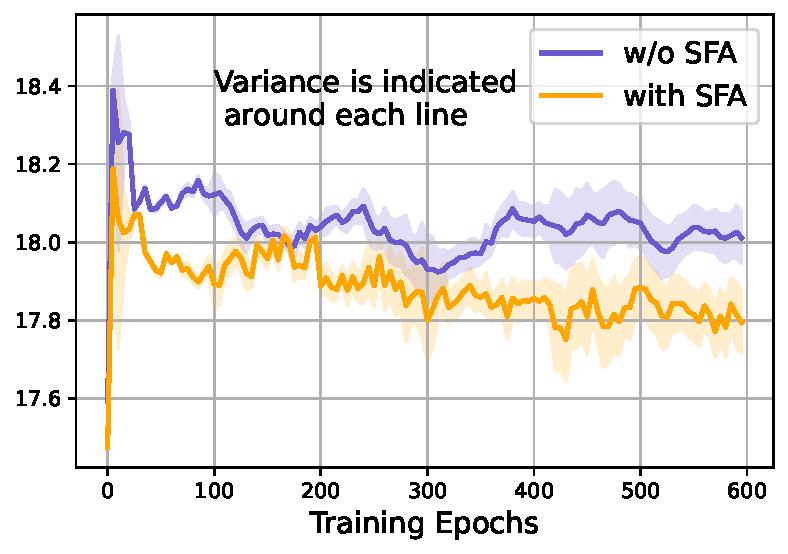
\includegraphics[width=\textwidth]{picture/alignment1.pdf}
\caption{CiteSeer}
\end{subfigure}
\hfill
\begin{subfigure}[b]{0.23\textwidth}
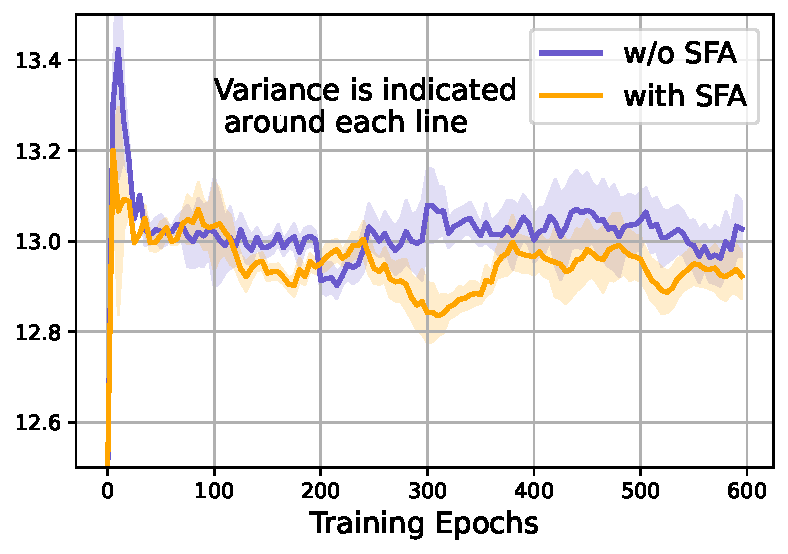
\includegraphics[width=\textwidth]{picture/alignment2.pdf}
\caption{WikiCS}
\end{subfigure}
\caption{Additional result on improved alignment on CiteSeer and WikiCS. Y-axis denote the alignment which is computed by $\|\mathbf{H}^\alpha -\mathbf{H}^\beta\|^2_F$ (or $\|\tilde{\mathbf{H}}^\alpha -\tilde{\mathbf{H}}^\beta\|^2_F$). The lower the curve the better.\label{fig:more_ima}}
\end{figure}

\section{Matrix Preconditioning}
\label{sec:mp}

% We believe there exist some misunderstanding of what our Eq. (3) does. Firstly, we typically use $k=1$ iterations of Alg. 1. Below we expand the most useful setting, $k=1$, to visualize how expanded Eq. (3) looks like:

%   $$ \tilde{\mathbf{H}}=\mathbf{H}\left(\mathbf{I} - \frac{\mathbf{H}^\top\mathbf{H}\mathbf{r}^{(0)}\mathbf{r}^{(0)\top}\mathbf{H}^\top\mathbf{H}}{\|\mathbf{H}^\top\mathbf{H}\mathbf{r}^{(0)}\|_2^2}\right),$$
%   where $\mathbf{r}^{(0)}\sim\mathcal{N}(0;{\bf I})$ is critical as it provides spectral noise injection.

%   The above expression shows there is never a need to use converged power iteration. On the contrary, we analyze/use properties of unconverged power iteration by multiplying feature matrix ${\bf H}$ with the complement of incomplete power iteration  to achieve flattening of spectrum according to Prop 3.2 with injected spectral noise according to Prop 3.3. 

%   Our method does not change the basis, i.e., in expectation, $\tilde{\bf H}$ and ${\bf H}$ enjoy the same basis which makes this method applicable to run over minibatches.
\begin{table}[h]
    \centering
    \resizebox{0.48\textwidth}{!}{
    \begin{tabular}{l|ccc}
    \toprule
           Method                     &   Cora        &  CiteSeer      &      PubMed   \\
      \midrule
         Matrix Precond. (by LU factorization) & $78.1 \pm0.2$       &$67.7\pm0.3$     & $83.4\pm0.1$    \\
      Grassman (w/o noise) ($\kappa=15$)       & $81.1 \pm0.2$       &$72.3\pm0.3$        & $83.2\pm0.2$    \\
      PCA                          & $80.0 \pm0.1$       &$70.5\pm0.5$     &$81.5\pm0.3$     \\    
      \rowcolor{LightCyan} SFA$_\text{infoNCE}$          &$\bf 86.43\pm0.1$    &$\bf 76.1\pm0.3$   &$\bf 86.2\pm0.2$ \\
      \bottomrule
    \end{tabular}
    }
    \caption{\label{tab:mp}Comparison of SFA with Matrix Precond., Grassman feature map, and PCA.}
\end{table}



\vspace{0.1cm}
\noindent\textbf{Matrix Preconditioning (MP).} For the discussion on Matrix Preconditioning (MP) techniques, ``Matrix Preconditioning Techniques and Applications'' book~\citelatex{chen2005matrix_sup} %by Ke Chen 
shows how to design an effective preconditioner matrix $\mathbf{M}$ in order to obtain a numerical solution for solving a large linear system: 
\begin{equation}
    \mathbf{Ax}=\mathbf{b} \rightarrow \mathbf{MAx}=\mathbf{Mb}
\end{equation}
The goal of Matrix Preconditioning is to make $\tilde{\mathbf{A}} = \mathbf{MA}$ to have small conditional number $p= \sigma_{\text{max}} / \sigma_{\text{min}}$, (\eg,  $\mathbf{M} \approx \mathbf{A^{-1}}$ and $\tilde{\mathbf{A}} \approx \mathbf{I}$) so that solving $\mathbf{MAx}=\mathbf{Mb}$ is much easier, faster and more accurate than solving $\mathbf{Ax}=\mathbf{b}$.

\vspace{0.1cm}
\noindent\textbf{Spectrum rebalancing via MP.} Since the $\tilde{\mathbf{A}}$ has small condition number $p= \sigma_{\text{max}} / \sigma_{\text{min}}$, MP may somehow achieve similar effect on balancing the spectrum. We set ${\bf A=\mathbf{H}^\top \mathbf{H}}$ as ${\bf A}$ is required to be SPD (needs to be invertible) which additionally complicates recovery of the rectangular feature matrix $\tilde{\bf H}$ from $\mathbf{MA}$. MP requires inversions for which backpropagation through SVD is unstable (SVD backpropagation fails under so-called non-simple eigenvalues due to undetermined solution). \\


Below we  provide clear empirical results and compare our method to Matrix Preconditioning, Grassman feature map (without noise injection) and PCA (Table~\ref{tab:mp}). Specifically: 
\begin{itemize}
    \item We recover the augmented feature $\tilde{\mathbf{H}}$ from $\tilde{\mathbf{H}}^\top \tilde{\mathbf{H}} = \mathbf{MH}^\top\mathbf{H}$ where the preconditioner $\mathbf{M} =\mathbf{U}^{-1} \mathbf{L}^{-1}$ (where $\mathbf{L}$, $\mathbf{U}$ is the LU factorization of $\mathbf{H}^\top\mathbf{H}$). 
    \item Judging from the role preconditioner ${\bf M}$ fulfills (fast convergence of the linear system), ${\bf M}$ cannot solve our problem, \ie, it cannot  flatten some $\kappa>0$ leading singular values (where signal most likely resides) while leaving remaining singular values unchanged (our method achieves that as Fig.~\ref{fig:sim2} of the main paper shows).
    \item Grassmann feature map which forms subspace from $\kappa>0$ leading singular values is in fact closer ``in principle'' to SFA than MP methods. Thus, we apply SVD and flatten $\kappa$ leading singular values $\sigma_i$ while nullifying remaining singular values $\sigma_i$. 
    \item We also compare our approach to PCA given the best $\kappa=20$ components.
\end{itemize}

The impact of subspace size $\kappa$ on results with Grassmann feature maps (without noise injection) is shown in Table~\ref{impact_subspace_size}. Number $\kappa=15$ agrees with our observations that leading 12 to 15 singular values should be flattened (Fig~\ref{fig:Eigen1} of the main paper). 

\vspace{0.2cm}
Our SFA performs better as:
\vspace{0.2cm}

\begin{itemize}
    \item It does not completely nullify non-leading singular values (some of them are still useful/carry signal).
    \item It does perform spectral augmentation on the leading singular values.
    \item  SFA does not rely on SVD whose backpropagation step is unstable (\eg, undefined for non-simple singular including zero singular values).
\end{itemize}
    
\begin{table}[h]
      \centering
      \resizebox{0.47\textwidth}{!}{
      \begin{tabular}{c|ccccccccc|c}
      \toprule
  $\kappa$ &2  & 5 & 10 & 15 & 20 & 30 &50 &100 & 250 &SFA$_\text{infoNCE}$ \\
  \midrule
           &$78.7$ &$80.1$ &$80.5$ &$81.1$ &$80.3$ &$80.5$ &$80.4$ &$80.2$ &$79.8$ & $\textcolor{blue}{\mathbf{86.4}}$\\
  \bottomrule
      \end{tabular}
      }
      \caption{\label{impact_subspace_size}Impact of subspace size $\kappa$ in Grassman feature map without the noise injection (Cora).}
\end{table}

It should be noted that most of random MP methods in \citelatex{halko2011finding_sup} need to compute the eigenvalues/eigenvectors which is time-consuming even with random SVD, and this performs badly in practice.  Suppose $k$ is the iteration number of a random approach, it then requires $O(kq)$ to get top $q$ eigenvectors (\eg, the random SVD in~\citelatex{halko2011finding_sup}). Then one must manually set eigenvectors to yield equal contribution (\ie, $\sigma_i=1$ for all $i$) which is what we do exactly for the Grassmann feature map in Table~\ref{impact_subspace_size}.
   

%


Other plausible feature balancing models which are outside of the scope of our work include the so-called democratic aggregation \citelatex{democratic_sup,Lin_2018_ECCV_sup}.

\section{Why does the Incomplete Iteration of SFA Work?~\label{sec:why_it_works}}

Let $\mathbf{M}=\mathbf{H}^\top\mathbf{H}$ and let the power iteration be expressed as $\mathbf{M}^k\mathbf{r}^{(0)}$ where $\mathbf{r}^{(0)}\sim\mathcal{N}(0;\mathbf{I})$, as in Algorithm \ref{algo:1}. Let $\mathbf{M}=\mathbf{V}\mathbf{\Sigma}^2\mathbf{V}^\top$ be an SVD of $\mathbf{M}$, then the eigenvalue decomposition admits $\mathbf{M}^{k}\mathbf{V}=\mathbf{V}\mathbf{\Sigma}^2$. Let $\mathbf{r}^{(0)}=\mathbf{V}\widetilde{\mathbf{r}}^{(0)}$ then $\mathbf{M}^{k}\mathbf{r}^{(0)}=\mathbf{M}^{k}\mathbf{V}\widetilde{\mathbf{r}}^{(0)}=\mathbf{V}\mathbf{\Sigma}^{2k}\widetilde{\mathbf{r}}^{(0)}$. We notice that
%
\begin{equation}
\begin{aligned}
    \mathbf{M}^{k}\mathbf{r}^{(0)}&=\sigma_1^{2k}\sum_i \mathbf{v}_i\Big(\frac{\sigma_i}{\sigma_1}\Big)^{2k}\widetilde{{r}}_i^{(0)}\\
  &=\sigma_1^{2k}\sum_i\mathbf{v}_i\Big(\frac{\sigma_i}{\sigma_1}\Big)^{2k} \langle\mathbf{v}_i^\top, \mathbf{r}^{(0)}\rangle\\
  &=\sum_i\gamma_i\mathbf{v}_i,
    \end{aligned}
\end{equation}
%
where $\gamma_i=\sigma_1^{2k}\big(\frac{\sigma_i}{\sigma_1}\big)^{2k} \langle\mathbf{v}_i^\top,\mathbf{r}^{(0)}\rangle$ which clearly shows that $\sum_i\gamma_i\mathbf{v}_i$ is a linear combination of more than one $\mathbf{v}_i$ if $k\ll\infty$. Notice also that as the smaller $\sigma_i$ is compared to the leading singular value $\sigma_1$, the quicker the ratio  $\Big(\frac{\sigma_i}{\sigma_1}\Big)^{2k}$ declines towards zero as $k$ grows (it follows the  power law non-linearity in Figure \ref{fig:mr}). Therefore, leading singular values make a significantly stronger contribution to the linear combination $\sum_i\gamma_i\mathbf{v}_i$ compared to non-leading singular values.
Thus, for small $k$, matrix
\begin{equation}
\mathbf{M}_{\text{PowerIter}}=\frac{\mathbf{M}^{k}\mathbf{r}^{(0)}{\mathbf{r}^{(0)}}^\top\mathbf{M}^{k}}{\lVert \mathbf{M}^{k}\mathbf{r}^{(0)}\rVert_2^2}=\frac{\big(\sum_i\rho_i\mathbf{v}_i\big)\big(\sum_j\rho_j\mathbf{v}_j^\top\big)}{\lVert\sum_l\rho_l\mathbf{v}_l\rVert_2^2},
\end{equation}
%
is a low-rank matrix ``focusing'' on leading singular vectors of $\mathbf{M}$ more according to the power law non-linearity in Figure \ref{fig:mr}. Intuitively, for that very reason, as a typical matrix spectrum of $\mathbf{H}$ (and $\mathbf{M}$) also follows the power law non-linearity, $\mathbf{H}$ is balanced by the inverted power law non-linearity of $\mathbf{I}-\mathbf{M}_{\text{PowerIter}}$.
%
In the above equation, $\rho_i=\big(\frac{\sigma_i}{\sigma_1}\big)^{2k} \langle\mathbf{v}_i^\top,\mathbf{r}^{(0)}\rangle$.

\begin{figure}
    \centering
    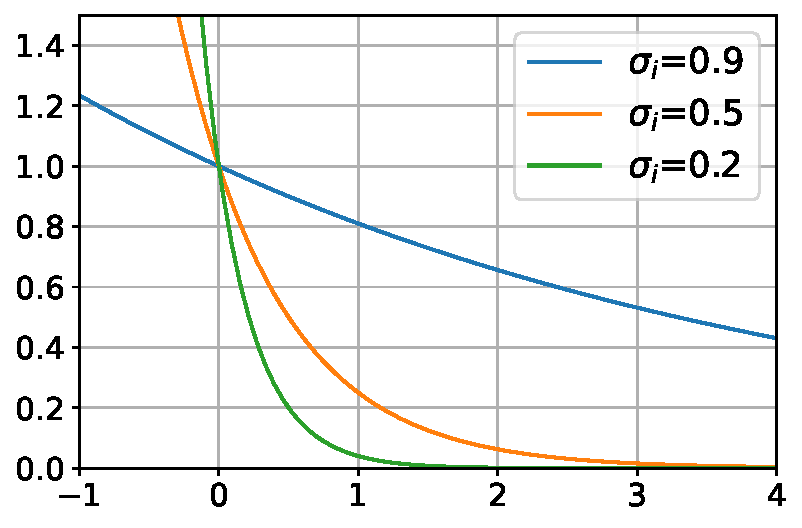
\includegraphics[width=0.35\textwidth]{picture/mr.pdf}
    \caption{Plot of $\big(\frac{\sigma_i}{\sigma_1}\big)^{2k}$ given $\sigma_1=1$ exhibits the power law non-linearity.\label{fig:mr}}
\end{figure}


\section{Broader Impact and Limitations}
Empowering deep learning with the ability of reasoning and making predictions on the graph-structured data is of broad interest, GCL may be applied in many applications such as recommendation systems, neural architecture search, and drug discovery. The proposed graph contrastive learning framework with spectral feature augmentations is a general framework that can improve the effectiveness and efficiency of graph neural networks through model pre-training. It can also inspire further studies on the augmentation design from a new perspective. Notably, our proposed SFA is a plug-and-play layer which can be easily integrated with existing systems (\eg, recommendation system) at a negligible runtime cost. SFA facilitates training of high-quality embeddings for users and items to resolve the cold-start problem in on-line shopping (and other graph-based applications). One limitation of our method is that our work mainly serves as a plug-in for existing machine learning models and thus it does not model any specific fairness prior. Thus, the GCL model with SFA is still required to prevent the bias of the model (\eg, gender bias, ethnicity bias, \etc), as the provided data itself may be strongly biased during the processes of the data collection, graph construction, \etc. Exploring the augmentation with some fairness prior may address such a limitation. We assume is reasonable to let the GCL model tackle the fairness issue. % rather than our single augmentation layer.





